\documentclass[
  man,
  floatsintext,
  longtable,
  nolmodern,
  notxfonts,
  notimes,
  colorlinks=true,linkcolor=blue,citecolor=blue,urlcolor=blue]{apa7}

\usepackage{amsmath}
\usepackage{amssymb}



\usepackage[bidi=default]{babel}
\babelprovide[main,import]{english}


% get rid of language-specific shorthands (see #6817):
\let\LanguageShortHands\languageshorthands
\def\languageshorthands#1{}

\RequirePackage{longtable}
% \setlength\LTleft{0pt}
\RequirePackage{threeparttablex}

% % 


\makeatletter
\renewcommand{\paragraph}{\@startsection{paragraph}{4}{\parindent}%
	{0\baselineskip \@plus 0.2ex \@minus 0.2ex}%
	{-.5em}%
	{\normalfont\normalsize\bfseries\typesectitle}}

\renewcommand{\subparagraph}[1]{\@startsection{subparagraph}{5}{0.5em}%
	{0\baselineskip \@plus 0.2ex \@minus 0.2ex}%
	{-\z@\relax}%
	{\normalfont\normalsize\bfseries\itshape\hspace{\parindent}{#1}\textit{\addperi}}{\relax}}
\makeatother




\usepackage{longtable, booktabs, multirow, multicol, colortbl, hhline, caption, array, float}
\setcounter{topnumber}{2}
\setcounter{bottomnumber}{2}
\setcounter{totalnumber}{4}
\renewcommand{\topfraction}{0.85}
\renewcommand{\bottomfraction}{0.85}
\renewcommand{\textfraction}{0.15}
\renewcommand{\floatpagefraction}{0.7}

\usepackage{tcolorbox}
\tcbuselibrary{listings,theorems, breakable, skins}
\usepackage{fontawesome5}

\definecolor{quarto-callout-color}{HTML}{909090}
\definecolor{quarto-callout-note-color}{HTML}{0758E5}
\definecolor{quarto-callout-important-color}{HTML}{CC1914}
\definecolor{quarto-callout-warning-color}{HTML}{EB9113}
\definecolor{quarto-callout-tip-color}{HTML}{00A047}
\definecolor{quarto-callout-caution-color}{HTML}{FC5300}
\definecolor{quarto-callout-color-frame}{HTML}{ACACAC}
\definecolor{quarto-callout-note-color-frame}{HTML}{4582EC}
\definecolor{quarto-callout-important-color-frame}{HTML}{D9534F}
\definecolor{quarto-callout-warning-color-frame}{HTML}{F0AD4E}
\definecolor{quarto-callout-tip-color-frame}{HTML}{02B875}
\definecolor{quarto-callout-caution-color-frame}{HTML}{FD7E14}

\newlength\Oldarrayrulewidth
\newlength\Oldtabcolsep


\usepackage{hyperref}




\providecommand{\tightlist}{%
  \setlength{\itemsep}{0pt}\setlength{\parskip}{0pt}}
\usepackage{longtable,booktabs,array}
\usepackage{calc} % for calculating minipage widths
% Correct order of tables after \paragraph or \subparagraph
\usepackage{etoolbox}
\makeatletter
\patchcmd\longtable{\par}{\if@noskipsec\mbox{}\fi\par}{}{}
\makeatother
% Allow footnotes in longtable head/foot
\IfFileExists{footnotehyper.sty}{\usepackage{footnotehyper}}{\usepackage{footnote}}
\makesavenoteenv{longtable}

\usepackage{graphicx}
\makeatletter
\newsavebox\pandoc@box
\newcommand*\pandocbounded[1]{% scales image to fit in text height/width
  \sbox\pandoc@box{#1}%
  \Gscale@div\@tempa{\textheight}{\dimexpr\ht\pandoc@box+\dp\pandoc@box\relax}%
  \Gscale@div\@tempb{\linewidth}{\wd\pandoc@box}%
  \ifdim\@tempb\p@<\@tempa\p@\let\@tempa\@tempb\fi% select the smaller of both
  \ifdim\@tempa\p@<\p@\scalebox{\@tempa}{\usebox\pandoc@box}%
  \else\usebox{\pandoc@box}%
  \fi%
}
% Set default figure placement to htbp
\def\fps@figure{htbp}
\makeatother


% definitions for citeproc citations
\NewDocumentCommand\citeproctext{}{}
\NewDocumentCommand\citeproc{mm}{%
  \begingroup\def\citeproctext{#2}\cite{#1}\endgroup}
\makeatletter
 % allow citations to break across lines
 \let\@cite@ofmt\@firstofone
 % avoid brackets around text for \cite:
 \def\@biblabel#1{}
 \def\@cite#1#2{{#1\if@tempswa , #2\fi}}
\makeatother
\newlength{\cslhangindent}
\setlength{\cslhangindent}{1.5em}
\newlength{\csllabelwidth}
\setlength{\csllabelwidth}{3em}
\newenvironment{CSLReferences}[2] % #1 hanging-indent, #2 entry-spacing
 {\begin{list}{}{%
  \setlength{\itemindent}{0pt}
  \setlength{\leftmargin}{0pt}
  \setlength{\parsep}{0pt}
  % turn on hanging indent if param 1 is 1
  \ifodd #1
   \setlength{\leftmargin}{\cslhangindent}
   \setlength{\itemindent}{-1\cslhangindent}
  \fi
  % set entry spacing
  \setlength{\itemsep}{#2\baselineskip}}}
 {\end{list}}
\usepackage{calc}
\newcommand{\CSLBlock}[1]{\hfill\break\parbox[t]{\linewidth}{\strut\ignorespaces#1\strut}}
\newcommand{\CSLLeftMargin}[1]{\parbox[t]{\csllabelwidth}{\strut#1\strut}}
\newcommand{\CSLRightInline}[1]{\parbox[t]{\linewidth - \csllabelwidth}{\strut#1\strut}}
\newcommand{\CSLIndent}[1]{\hspace{\cslhangindent}#1}


\usepackage[nolongtablepatch]{lineno}
\linenumbers



\usepackage{newtx}

\defaultfontfeatures{Scale=MatchLowercase}
\defaultfontfeatures[\rmfamily]{Ligatures=TeX,Scale=1}





\title{Testing the Relationship between Phenomenological Control related
to Illusion Sensitivity}
\shorttitle{Illusion Sensitivity and Phenomenological Control}


\usepackage{etoolbox}







\authorsnames{Dominique Makowski,Ana Neves}




\affiliation{
{School of Psychology, University of Sussex}}






\leftheader{Makowski and Neves}



\abstract{Visual illusions highlight how easily our conscious experience
can be altered with respect to perceptual reality. Despite sharing
in-principle mechanisms with phenomenological control, i.e., the ability
to alter our perceptual experience to match task demands or
expectations, research tying the two remains scarce. This study aims to
replicate and expand Lush et al.~(2022) reporting an absence of
correlation between phenomenological control (measured using the
Phenomenological Control Scale) and illusion sensitivity to different
illusion types. \emph{{[}N participants were recruited in an online
study. Results will be added in the final version of the
manuscript{]}}.}
% 
\keywords{illusion sensitivity, visual illusions, phenomenological
control, suggestibility, hypnotizability}

\authornote{\par{\addORCIDlink{Dominique
Makowski}{0000-0001-5375-9967}}\par{\addORCIDlink{Ana
Neves}{0009-0006-0020-7599}}
\par{ }
\par{       Author roles were classified using the Contributor Role Taxonomy (CRediT; https://credit.niso.org/) as follows: Dominique
Makowski:   Conceptualization, Data curation, formal Analysis, Funding
acquisition, Investigation, Methodology, Project
administration, Resources, Software, Supervision, Validation, Visualization, Writing
-- original draft, Writing -- review \& editing; Ana Neves:   Project
administration, Data curation, Formal
Analysis, Investigation, Visualization, Writing -- original
draft, Writing -- review \& editing}
\par{Correspondence concerning this article should be addressed
to Dominique Makowski, Email: D.Makowski@sussex.ac.uk}
}


\makeatletter
\let\endoldlt\endlongtable
\def\endlongtable{
\hline
\endoldlt
}
\makeatother

\urlstyle{same}



% From https://tex.stackexchange.com/a/645996/211326
%%% apa7 doesn't want to add appendix section titles in the toc
%%% let's make it do it
\makeatletter
\xpatchcmd{\appendix}
  {\par}
  {\addcontentsline{toc}{section}{\@currentlabelname}\par}
  {}{}
\makeatother

\begin{document}

\maketitle


\setcounter{secnumdepth}{-\maxdimen} % remove section numbering

\setlength\LTleft{0pt}

\resetlinenumber[1]



Visual Illusions are an interesting type of stimuli highlighting the
ease with which our phenomenological conscious experience can become
dissociated from physical reality. Their robust and reliable effect
makes them useful stimuli to explore how perception is constructed and
shaped, and several theoretical models have been put forth to explain
how they work. \textbf{In particular, illusions have been reframed using
a predictive coding account of perception (e.g., Notredame et al., 2014;
Nour \& Nour, 2015)} in which the brain optimally combines, using some
flavour of Bayesian inference, perceptual inputs with prior knowledge to
make sense of ambiguous environments (Friston, 2010).

Such computational model(s) propose to conceptualize illusions as
stimuli providing weak or conflicting sensory evidence (Gershman et al.,
2012; Sundareswara \& Schrater, 2008) that bias perception toward prior
knowledge. In other words, the weight of priors, in the form of
perceptual knowledge about the world (e.g., internalized rules of
perspective) is amplified when the sensory input is confusing. For
instance, in the Müller-Lyer illusion, we ``compute'' the two (actually
identical) lines as being of different lengths because the line flanked
with converging fins is misinterpreted as being further away (Notredame
et al., 2014). In this context, measuring sensitivity to illusion can be
operationalized as indexing the parameters of the Bayesian inference
process (e.g., prior precision).

These accounts also provide a compelling framework to explain existing
findings reporting interindividual variability in the sensitivity to
illusions. Indeed, several studies suggest a potential link with
psychopathology, in particular schizophrenia (Costa et al., 2023) and
autism (Gori et al., 2016), in which the reported lower sensitivity to
illusions has been attributed to a diminished influence of top-down
processes such as prior knowledge (Mitchell et al., 2010) and a greater
emphasis on (i.e., precision of) sensory information (Palmer et al.,
2017). Evidence beyond psychopathology also suggests variability in the
general population, potentially correlated with personality traits such
as agreeableness and honest-humility (Makowski et al., 2023), as well as
cognitive abilities (Shoshina \& Shelepin, 2014).

However, the exact nature of this interindividual variability and its
potential origin remains unclear. The somewhat mixed evidence in the
literature regarding its generalizability and strength could be related
to the variety of the paradigms used and the type of processes being
mobilised (Makowski et al., 2021). Indeed, traditional methods
frequently focus on participant's experience by prompting them to assess
the difference between two identical targets, estimate the target's
physical properties, or adjust the targets to match a reference stimulus
(Todorović, 2020). Relying on metacognitive judgments about one's
subjective experiences adds an additional layer to the measure that
might not be desired when attempting to measure illusion
\textbf{sensitivity}. Moreover, paradigms often face challenges in
diversifying the illusory effects (i.e., using multiple stimuli to
experimentally manipulate the strength of the illusion) and the illusion
types (i.e., using various illusions, such as Müller-Lyer, Ebbinghaus,
Delboeuf which might rely on a different admixture of mechanisms),
hindering the potential of obtaining a comprehensive, valid, and
reliable measure of illusion sensitivity.

\begin{figure}

\caption{\label{fig-illusion_framework}The parametric framework for
visual illusions (Makowski et al., 2021) applied to the Müller-Lyer
illusion. Below are examples of stimuli showcasing the manipulation of
two parameters, task difficulty and illusion strength.}

\centering{

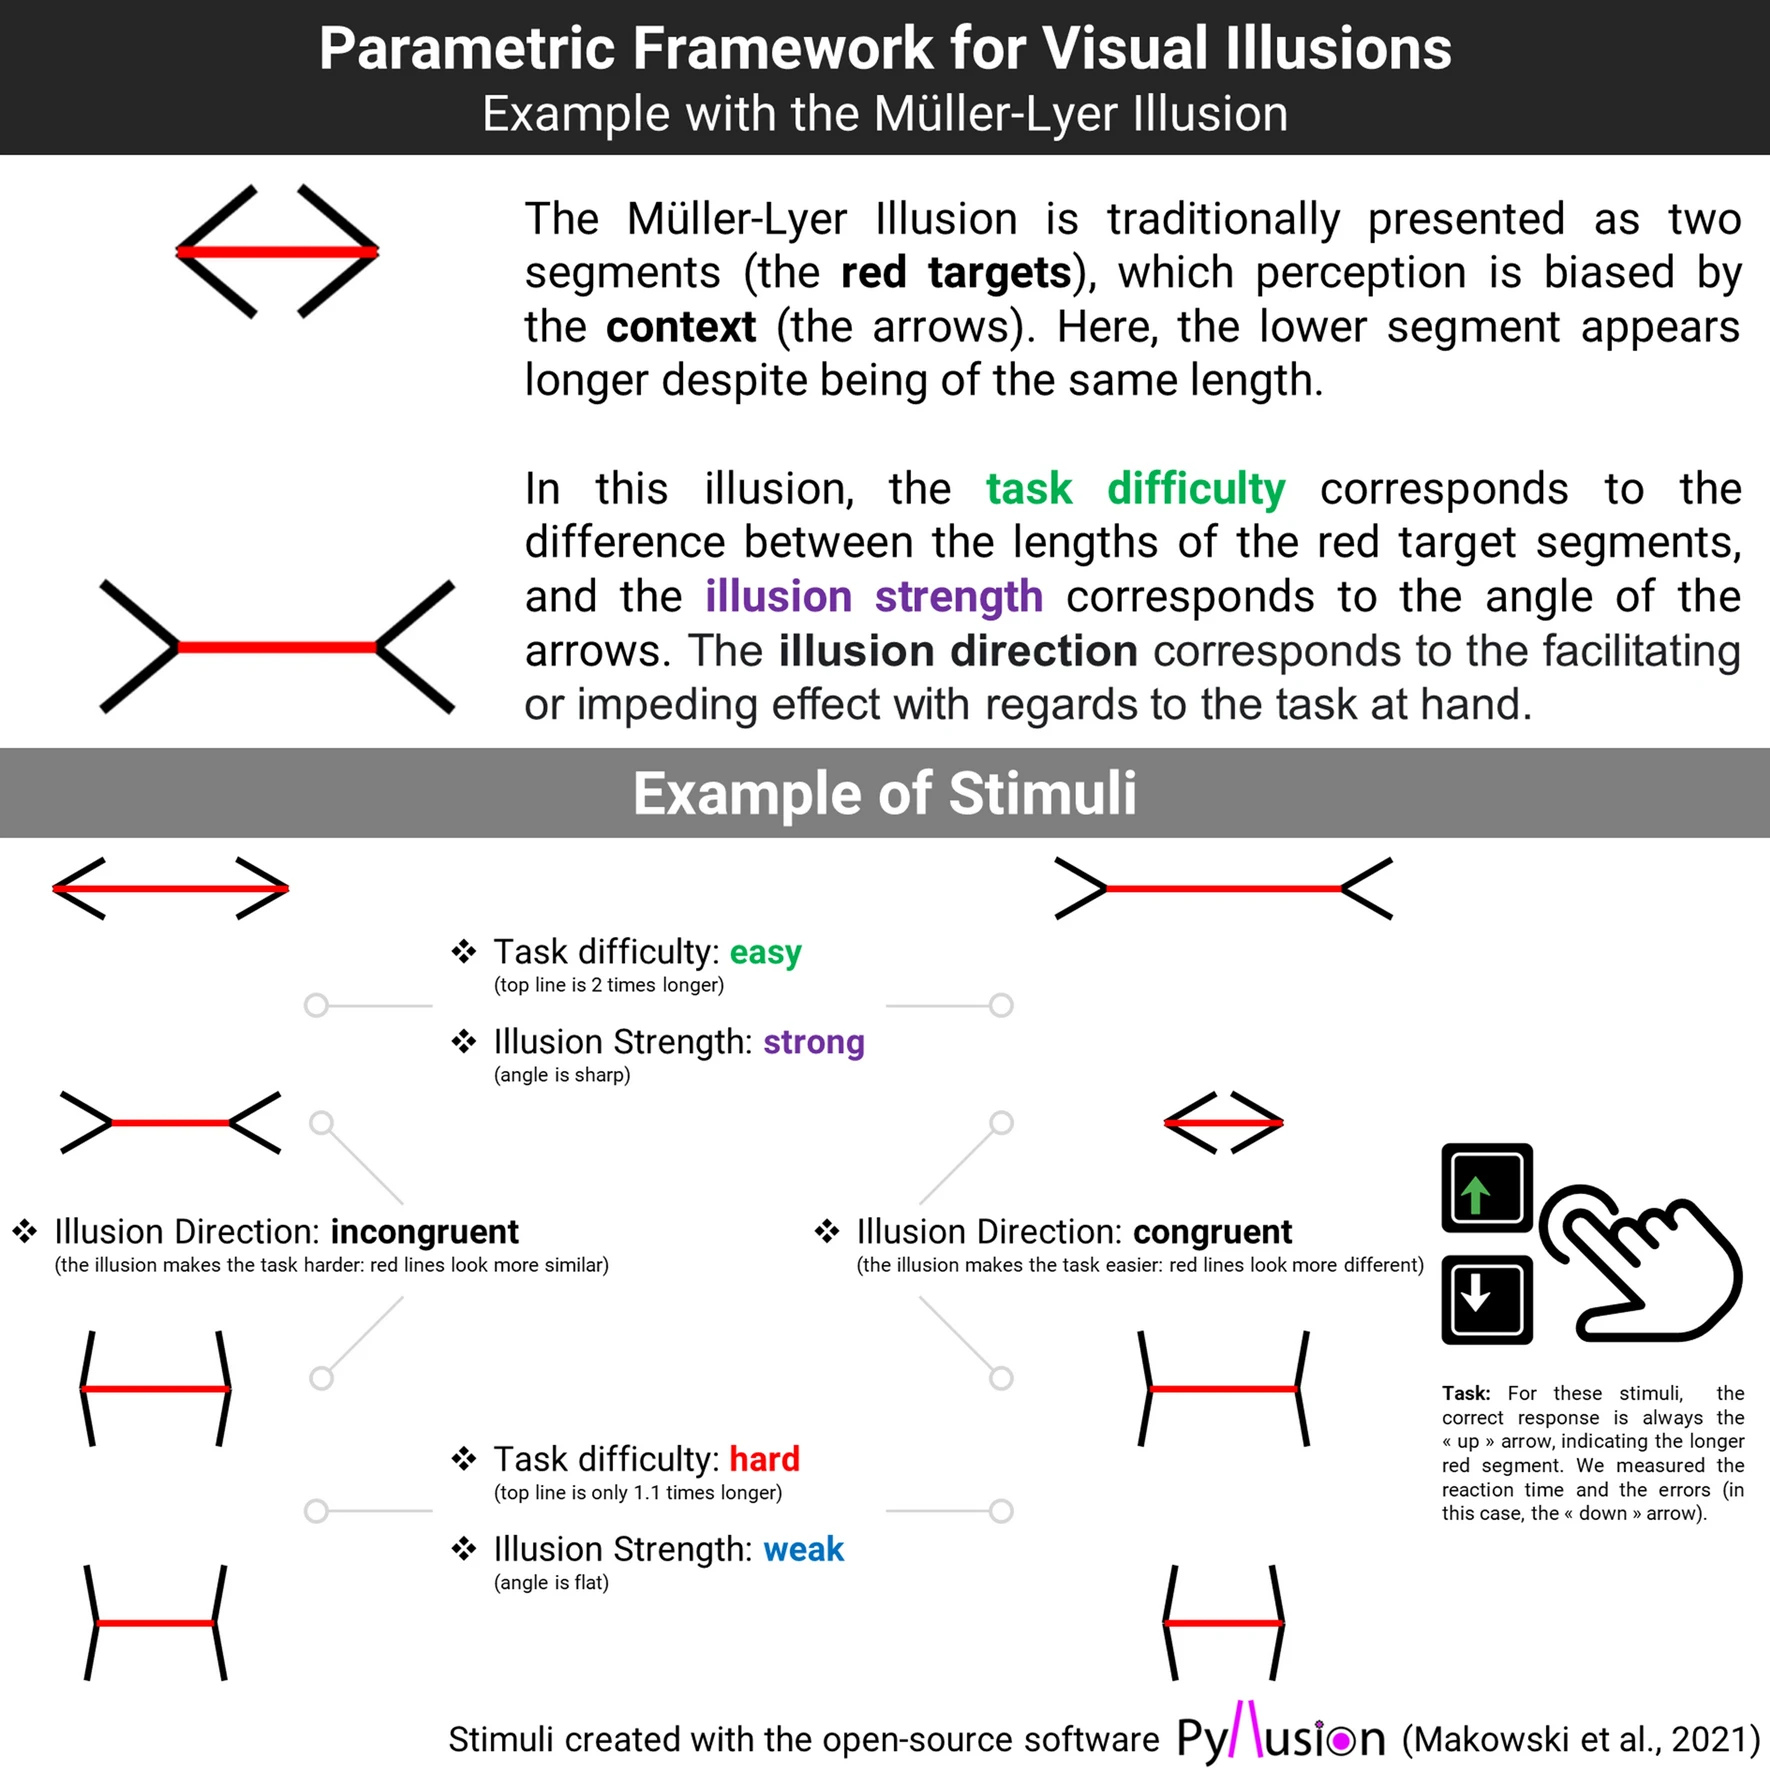
\includegraphics[width=1\linewidth,height=\textheight,keepaspectratio]{img/IG_framework.png}

}

\end{figure}%

The ``Illusion Game'' paradigm (Makowski et al., 2023) has been recently
developed to measure illusion sensitivity to various illusion types
through its behavioural impact (on response time and error rate) in a
perceptual decision task (where participants have to respond as fast as
possible; e.g., ``which of the left or right circles is bigger''). The
stimuli for different classical illusions are created using the
\emph{Pyllusion} software (Makowski et al., 2021), which allows
researchers to modulate the strength of the illusion as a continuous
dimension, independently from the difficulty of the perceptual task (see
Figure~\ref{fig-illusion_framework}). This paradigm, inspired by
psychophysics, lends itself to the computational modelling of illusion
sensitivity through its \textbf{interference effect ---an effect that
disrupts an individual's ability to accurately discriminate between
perceptual stimuli.} \textbf{This approach aims to bypass some of the
metacognitive processes involved in other paradigms, offering a more
direct and objective measure of how illusions influence perceptual
judgment.}

Interestingly, the fact that inter-individual variability in illusion
sensitivity seems to persist in this task suggests that it is not solely
explained by \textbf{metacognitive ability differences}, and gives rise
to the following question: is the variability in illusion sensitivity
related to low-level perceptual processes (e.g., baseline precision of
perceptual priors), or rather to the ability to actively control and
``resist'' the illusion in order to achieve the task at hand
(higher-level modulation of the perceptual inference parameters). If the
latter is true, then illusion sensitivity measured in contexts with
strong task-demand characteristics, e.g., in paradigms where
participants' performance is explicitly or implicitly assessed (i.e.,
where there is an incentive to downplay the illusion effect) might
correlate with one's ability to alter one's subjective experience
following suggestions - a mechanism referred to as ``phenomenological
control''.

The idea that we are endowed with the potential to unconsciously alter
our subjective experience and distort reality - even momentarily - to
meet the goals at hand is not novel. While this phenomenon has been
historically often studied under the label of ``hypnotisability'' - the
tendency to alter our conscious experience to match external demands
(Lush et al., 2021), the term ``phenomenological control'' (PC) has been
recently introduced to disconnect this concept from the potentially
negative associations with hypnosis and the misconception that a
hypnotic context is necessary for responding to imaginative suggestions
(Dienes et al., 2022).

To encourage the empirical exploration of our ability and tendency to
alter our phenomenological experience and further accelerate
investigations away from the hypnotic context, Lush et al. (2021)
adapted the Sussex-Waterloo Scale of Hypnotisability (SWASH, Lush et
al., 2018) by removing all its references to hypnosis, to measure trait
phenomenological control. \textbf{This newly developed phenomenological
control scale (PCS) consists of 10 imaginative suggestions followed by
subjective ratings for each suggestion and has demonstrated validity in
online experiments (Lush et al., 2022).}

Interestingly, Lush et al. (2022) did test for a relationship between PC
and illusion sensitivity using the Müller-Lyer illusion (in which the
arrangement of the arrowheads flanking two lines makes them appear as
having different lengths), and reported evidence in favour of an absence
of correlation between the two measures. This finding was interpreted as
indicative of the cognitive impenetrability of illusions, implying that
the effect is driven by low-level processes and therefore not influenced
by top-down mechanisms such as PC. \textbf{Note that both
prior-knowledge and phenomenological control are considered top-down
processes, but the cognitive impenetrability hypothesis suggests that
the processes at stake for the illusions happen at a lower-
encapsulated- level (in the form of \emph{perceptual} priors)}.

The goal of this study is thus to replicate the results from Lush et al.
(2022) pointing to an absence of a relationship between phenomenological
control and illusion sensitivity, by generalising them to a different
illusion paradigm that encompasses other illusion types.
\textbf{Additionally, we will explore the relationship between
psychoticism, as a proxy for schizophrenia, and illusion sensitivity to
assess the potential impact of lower-level effects---such as weak priors
observed in individuals with schizophrenia (Costa et al., 2023)---on
sensitivity to illusions.} \textbf{These analyses may offer evidence
clarifying whether inter-individual variability in illusion sensitivity
is driven by lower-level perceptual mechanisms or higher-level cognitive
processes (Table~\ref{tbl-DesignTable}).}

\begin{table}

{\caption{{Study Design Table}{\label{tbl-DesignTable}}}
\vspace{-20pt}}

\global\setlength{\Oldarrayrulewidth}{\arrayrulewidth}

\global\setlength{\Oldtabcolsep}{\tabcolsep}

\setlength{\tabcolsep}{2pt}

\renewcommand*{\arraystretch}{1.5}



\providecommand{\ascline}[3]{\noalign{\global\arrayrulewidth #1}\arrayrulecolor[HTML]{#2}\cline{#3}}

\begin{longtable*}[c]{cc}



\ascline{0.75pt}{000000}{1-2}

\multicolumn{1}{>{}c}{\textcolor[HTML]{000000}{\fontsize{11}{22}\selectfont{\global\setmainfont{Times New Roman}{\textbf{Question}}}}} & \multicolumn{1}{>{}c}{\textcolor[HTML]{000000}{\fontsize{11}{22}\selectfont{\global\setmainfont{Times New Roman}{Is\ there\ a\ correlation\ between\ trait\ phenomenological\ control\ (PC)\ and\ visual\ illusion\ (VI)\ sensitivity?\ Additionally,\ is\ there\ a\ relationship\ between\ VI\ sensitivity\ and\ the\ psychoticism\ facet\ of\ the\ PID-5,\ as\ a\ proxy\ for\ schizophrenia-related\ traits?}}}} \\





\multicolumn{1}{>{}c}{\textcolor[HTML]{000000}{\fontsize{11}{22}\selectfont{\global\setmainfont{Times New Roman}{\textbf{Hypothesis}}}}} & \multicolumn{1}{>{}c}{\textcolor[HTML]{000000}{\fontsize{11}{22}\selectfont{\global\setmainfont{Times New Roman}{In\ line\ with\ Lush\ et\ al.\ (2022),\ we\ hypothesise\ that\ there\ will\ be\ evidence\ supporting\ the\ absence\ of\ a\ relationship\ between\ PC\ and\ VI\ sensitivity.\ Based\ on\ Makowski\ et\ al.\ (2023)\ and\ prior\ work\ on\ weak\ priors\ in\ schizophrenia,\ we\ hypothesise\ that\ higher\ psychoticism\ scores\ will\ be\ positively\ associated\ with\ VI\ sensitivity.}}}} \\





\multicolumn{1}{>{}c}{\textcolor[HTML]{000000}{\fontsize{11}{22}\selectfont{\global\setmainfont{Times New Roman}{\textbf{Sampling\ Plan}}}}} & \multicolumn{1}{>{}c}{\textcolor[HTML]{000000}{\fontsize{11}{22}\selectfont{\global\setmainfont{Times New Roman}{The\ goal\ is\ to\ recruit\ around\ 500\ adult\ English\ speakers\ using\ Prolific.\ This\ sample\ size\ is\ based\ on\ the\ ones\ used\ in\ Lush\ et\ al.,\ 2021\ and\ Lush\ et\ al.,\ 2022\ that\ we\ aim\ at\ replicate.}}}} \\





\multicolumn{1}{>{}c}{\textcolor[HTML]{000000}{\fontsize{11}{22}\selectfont{\global\setmainfont{Times New Roman}{\textbf{Analysis\ Plan}}}}} & \multicolumn{1}{>{}c}{\textcolor[HTML]{000000}{\fontsize{11}{22}\selectfont{\global\setmainfont{Times New Roman}{BBayesian\ correlations\ will\ be\ conducted\ using\ the\ BayesFactor::correlationBF()\ function,\ with\ a\ medium\ prior\ (r-scale\ =\ 1/3),\ separately\ for:\ 1)\ PC\ scores\ and\ VI\ sensitivity\ (error\ rate\ and\ IES),\ across\ all\ three\ illusion\ types.\ 2)\ Psychoticism\ facet\ scores\ from\ the\ PID-5\ and\ VI\ sensitivity\ scores,\ across\ all\ three\ illusion\ types.}}}} \\





\multicolumn{1}{>{}c}{\textcolor[HTML]{000000}{\fontsize{11}{22}\selectfont{\global\setmainfont{Times New Roman}{\textbf{Rationale\ for\ Deciding\ the\ Sensitivity\ of\ the\ Test}}}}} & \multicolumn{1}{>{}c}{\textcolor[HTML]{000000}{\fontsize{11}{22}\selectfont{\global\setmainfont{Times New Roman}{For\ the\ PC–VI\ sensitivity\ relationship,\ we\ will\ interpret\ BF₁₀\ ≤\ 1/3\ as\ evidence\ against\ a\ relationship,\ in\ line\ with\ Lush\ et\ al.\ (2022).\ For\ the\ psychoticism–VI\ sensitivity\ relationship,\ BF₁₀\ >\ 3\ will\ be\ interpreted\ as\ evidence\ supporting\ a\ relationship,\ following\ findings\ by\ Makowski\ et\ al.\ (2023).}}}} \\





\multicolumn{1}{>{}c}{\textcolor[HTML]{000000}{\fontsize{11}{22}\selectfont{\global\setmainfont{Times New Roman}{\textbf{Interpretation\ Given\ Different\ Outcomes}}}}} & \multicolumn{1}{>{}c}{\textcolor[HTML]{000000}{\fontsize{11}{22}\selectfont{\global\setmainfont{Times New Roman}{If\ there\ is\ no\ evidence\ for\ a\ PC–VI\ relationship\ across\ all\ three\ illusions,\ it\ would\ support\ the\ hypothesis\ that\ VI\ sensitivity\ is\ independent\ from\ PC.\ If\ a\ positive\ association\ is\ found\ between\ psychoticism\ and\ VI\ sensitivity,\ it\ may\ suggest\ a\ low-level\ perceptual\ basis\ for\ inter-individual\ differences\ in\ illusion\ sensitivity.}}}} \\





\multicolumn{1}{>{}c}{\textcolor[HTML]{000000}{\fontsize{11}{22}\selectfont{\global\setmainfont{Times New Roman}{\textbf{Theory\ That\ Could\ Be\ Shown\ Wrong\ by\ the\ Outcomes}}}}} & \multicolumn{1}{>{}c}{\textcolor[HTML]{000000}{\fontsize{11}{22}\selectfont{\global\setmainfont{Times New Roman}{The\ cognitive\ impenetrability\ of\ visual\ illusions,\ which\ posits\ that\ illusion\ sensitivity\ is\ driven\ solely\ by\ low-level\ processes\ and\ is\ not\ influenced\ by\ top-down\ mechanisms\ such\ as\ phenomenological\ control.\ Conversely,\ a\ lack\ of\ association\ with\ psychoticism\ would\ challenge\ the\ view\ that\ low-level\ perceptual\ alterations\ underlie\ illusion\ sensitivity\ in\ non-clinical\ populations.}}}} \\

\ascline{0.75pt}{000000}{1-2}



\end{longtable*}



\arrayrulecolor[HTML]{000000}

\global\setlength{\arrayrulewidth}{\Oldarrayrulewidth}

\global\setlength{\tabcolsep}{\Oldtabcolsep}

\renewcommand*{\arraystretch}{1}

\end{table}

\section{Methods}\label{methods}

\subsection{Participants}\label{participants}

We aim to recruit around 500 (in line with the sample sizes used in Lush
et al., 2021; Lush et al., 2022) adult English native speakers with a
desktop device using Prolific (www.prolific.co). Participants will be
first presented with an explanatory statement and the consent form, and
can proceed by pressing a button to confirm they have read and
understood the information. This study has been approved by the ethics
board of the School of Psychology of the University of Sussex
(ER/ASF25/5).

\subsection{Procedure}\label{procedure}

The experiment's setup follows of the born-open principle (De Leeuw,
2023). The online experiment, implemented entirely using JsPsych (De
Leeuw, 2015), has its code stored on GitHub and will leverage the power
of the platform to host the experiment for free. Participant's raw data
files (containing identifiers) \textbf{are} automatically stored in a
private OSF repository. The preprocessing and analysis scripts, as well
as the anonymized data, will be available directly on GitHub, ensuring
the transparency and reproducibility of all the analysis steps.

Participants will be presented with a consent form followed by
demographic questions (gender, education level, age, and ethnicity).
\textbf{Although these variables are not directly analyzed in the
current study, they will be used to provide to provide a detailed and
thorough description of the sample and maximizing data reusability.}
\textbf{Participants will then be administered the PCS and the Illusion
Game task (IG) in a counterbalanced order.}

\subsubsection{Phenomenological Control Scale
(PCS)}\label{phenomenological-control-scale-pcs}

Participants will be asked to put on their headphones and await further
auditory instructions. The PCS procedure starts with a recorded
introduction explaining that a series of tests will be applied to
evaluate how experiences can be created through imagination. This will
be followed by 10 suggestions in a fixed order (see Lush et al., 2021),
such as ``now extend your arms ahead of you, with palms facing each
other, hands about a foot apart'' and ``as you sit comfortably in your
chair with your eyes closed, a picture of two balls will be displayed on
the computer screen''. \textbf{Once the 10 suggestions are completed,
participants will be asked to rate their subjective experiences and
response to each suggestion on a 6-points Likert scale (from 0-5).}
Phenomenological control will be indexed by averaging the scores from
the 10 scales.

\subsubsection{Illusion Game}\label{illusion-game}

The task is an adaptation of the one used in Makowski et al. (2023) to
make it shorter, in which participants must make perceptual judgments
(e.g., ``which red line is the longer'') as quickly and accurately as
possible. It includes 3 illusion types, namely Ebbinghaus, Müller-Lyer,
and Vertical-Horizontal (see Figure~\ref{fig-illusionexample}).

\begin{figure}

\caption{\label{fig-illusionexample}The study involved three visual
illusions, in which participants were instructed to respond as quickly
as possible without making errors. Each illusion included two
manipulated parameters: strength (e.g., the angle of the outward- or
inward-pointing arrow-like fins in the Müller-Lyer illusion) and
difficulty (e.g., the difference in line lengths in the Müller-Lyer
illusion).}

\centering{

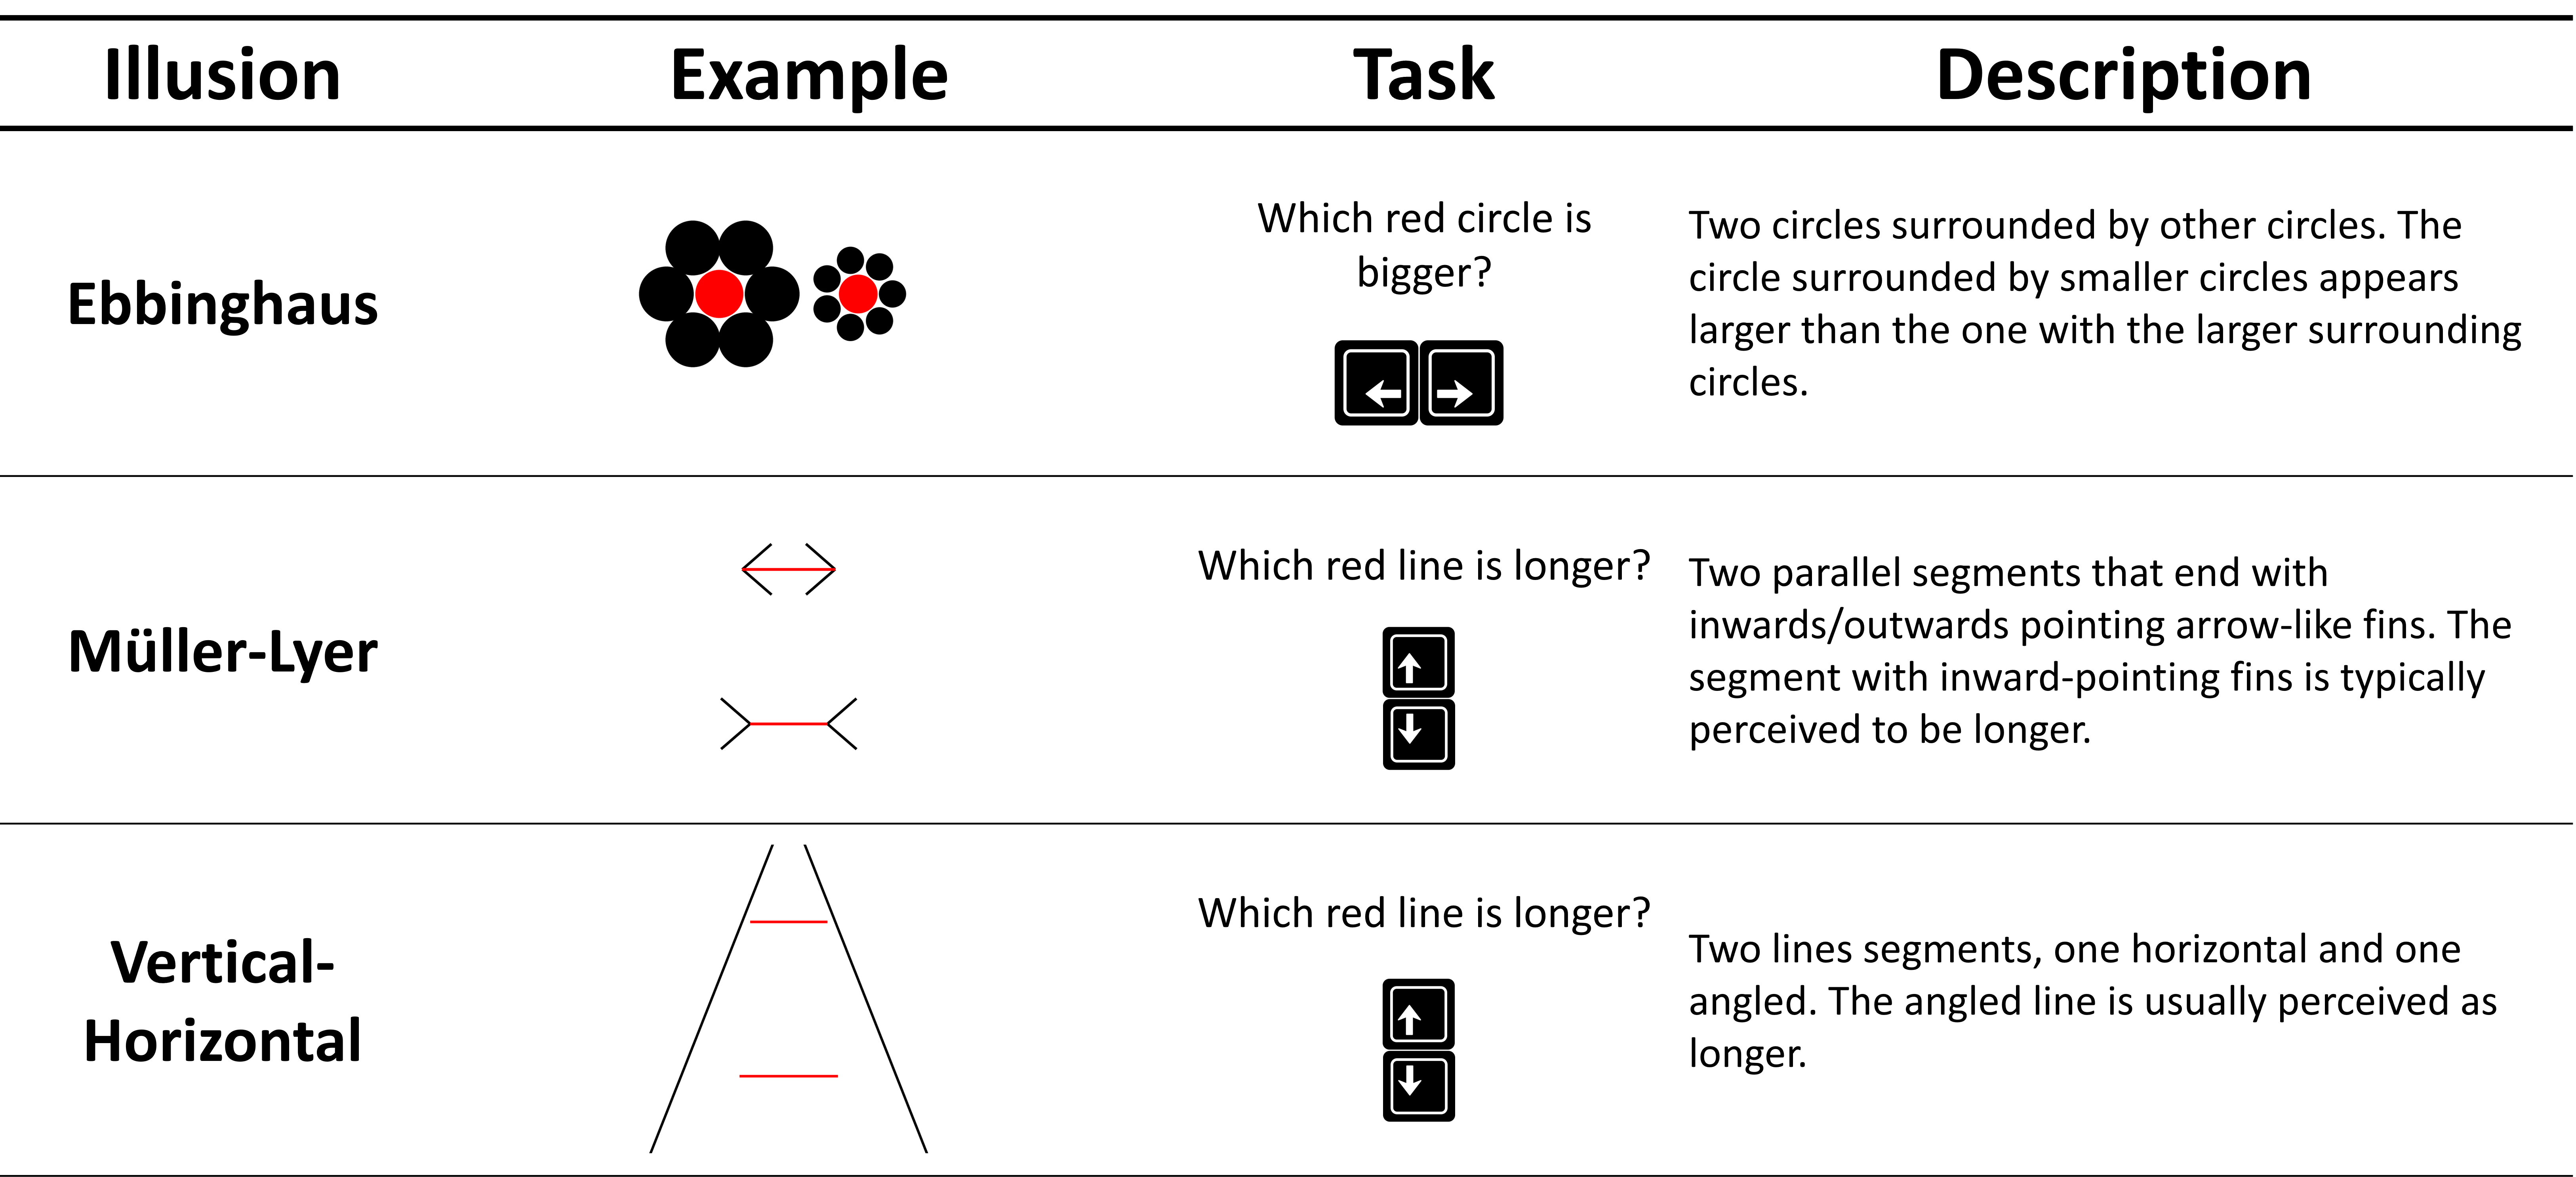
\includegraphics[width=1\linewidth,height=\textheight,keepaspectratio]{img/IllusionTable.jpg}

}

\end{figure}%

\textbf{In the original Illusion Game, 10 visual illusions were
presented in two sets, following a practice trial, and separated by two
short questionnaires. Participants completed a total of 1,340 trials,
with the experiment lasting approximately 55 minutes.} \textbf{In the
current procedure, only three illusions are used, selected based on the
original study's findings that these illusions most strongly contribute
to illusion sensitivity.}

The procedure encompasses 2 sets of 80 trials for each illusion type,
\textbf{preceded by a practice trial for each illusion}. Each set will
include, in a random order, the 3 blocks of illusion types, in which
trials are separated by a fixation cross, temporally (uniformly sampled
duration of 500 - 1000s) and spatially jittered (around the centre of
the screen in a radius of a 1 cm) to attenuate its potential usefulness
as a reference point. After each illusion type block, an arbitrary score
is presented (computed as a scaled Inverse Efficiency Score) as a
gamification mechanism to increase motivation to perform to the best of
one's abilities. To mitigate for the potential variability in the
speed/accuracy trade-off, the instructions emphasize with equal weight
to be fast and to avoid errors.

For each illusion type, two continuous dimensions are orthogonally
manipulated namely task difficulty and illusion strength, so that each
trial corresponds to a unique combination, \textbf{providing an
objectively correct answer for each task.} \textbf{The use of these
manipulations allows concise, standardised reporting of illusion
parameters and ensures our stimuli are fully reproducible (see Makowski
et al., 2021).}

Task difficulty corresponds to the difficulty of the perceptual decision
(e.g., if the task is to select the longest red line, task difficulty
corresponds to how the lines are objectively different). Illusion
strength corresponds to the degree to which the illusion elements (e.g.,
the black arrow lines in Müller-Lyer) are interfering with the
aforementioned task. Note that the illusion effect can be either
``incongruent'', \textbf{making the task more difficult by biasing
perceptual decisions toward the incorrect response} or ``congruent'',
\textbf{making the task easier by biasing decisions toward the correct
response (e.g., in the Müller-Lyer illusion, if the outwards-facing
arrowheads are placed on the longer line, identifying which line is the
longest becomes easier)}. Participants respond with a key arrow (left
vs.~right; or up vs.~down), and their reaction time (RT) and accuracy
are recorded.

Visual illusion sensitivity will be measured as the average error rate
in the incongruent condition, and separately for the 3 illusion types.
Although the error rate is arguably a crude score, which does not take
into account the effect of varying illusion strength, the interaction
with task difficulty and the possible adjustments in response strategy
(speed-accuracy trade off), it is also the most simple and easy to
reproduce, hence its usage as our primary outcome for the current
\textbf{registered report}. \textbf{As a secondary exploratory outcome,
the Inverse Efficiency Score (IES, Townsend \& Ashby, 2014) will also be
computed. This metric incorporates both speed and accuracy by dividing
the mean reaction time of correct responses by the proportion of correct
responses, separately for each illusion.}

The two sets of 3 illusion blocks will be separated by 2 short
questionnaires acting as a break, namely the IPIP-6 (Sibley et al.,
2011), measuring 6 personality traits with 24 analogue scales items, and
the PID-5 (Krueger et al., 2011), measuring 5 maladaptive personality
traits with 25 Likert scales items. These questionnaires are included as
a way of providing a break between the two cognitively taxing blocks and
maintain paradigmatic consistency with previous studies (Makowski et
al., 2023). \textbf{Additionally, the psychoticism subscale of the PID-5
will be used to examine the correlation between maladaptive traits and
illusion sensitivity, evaluating the existence of the link proposed in
previous studies (Costa et al., 2023).}

\subsection{Data Analysis}\label{data-analysis}

The PCS will contain several manipulation check indices to identify
problematic participants. \textbf{The phenomenological control task
consists of various auditory and visual exercises.} \textbf{At the start
of the task, participants first hear someone say ``hello.'' They are
then asked to choose from several options, including ``Hello,''
``Goodbye,'' ``How are you,'' and ``Thank you''.} \textbf{Any
participant who selects an option other than the correct one will be
considered inattentive} \textbf{In another exercise, participants
receive the following instruction: ``Open your eyes. You will see only
two balls on the screen\ldots just two balls''.} \textbf{However, three
differently coloured balls are actually displayed.} \textbf{If
participants select the option ``no balls were shown'', it indicates
they failed to pay attention to both the auditory instructions and the
visual stimuli.} \textbf{Lastly, in another exercise, participants are
asked to press the spacebar six times.} \textbf{If they press it fewer
than five times within the allotted time, it suggests a lack of
attentiveness to the auditory instructions.} \textbf{Participants will
be excluded if they fail at least one of these checks.} \textbf{Lastly,
reliability of the PCS will be assessed by computing Cronbach's alpha
(Cronbach, 1951).}

\textbf{To assess whether the illusions functioned as expected, stimuli
will be categorized into three groups: Strong Illusion Strength \&
Incongruent, Mild Illusion Strength \& Incongruent, and Congruent.}
\textbf{Two Bayesian t-tests will be conducted to assess differences in
IES between the Congruent and Mild conditions, and between the Mild and
Strong conditions.} \textbf{Significant differences in these comparisons
will provide evidence that the illusions functioned as intended.}

\textbf{The two outcome measures---error rate and IES---will be computed
for each illusion and for each illusion strength group: Strong Illusion
Strength \& Incongruent, Mild Illusion Strength \& Incongruent, and
Congruent.} \textbf{Correlation will be computed between the mild and
strong groups for each illusion and outcomes separately.} \textbf{If
these correlations are high (\emph{r} \textgreater{} .50, Cohen, 2013),
the mild and strong illusion strength groups will be collapsed and the
outcomes will be recomputed across all trials, otherwise they will be
treated as separate in subsequent analyses.}

\textbf{Reliability analyses will then be conducted on all resulting
indices.} \textbf{First, split-half reliability, to assess internal
consistency, will be computed by correlating two equal subsets of
individual scores, with high correlations expected (\emph{r}
\textgreater{} .5).} \textbf{Second, inter-illusion reliability will be
evaluated using Cronbach's alpha across the three illusions.}

Illusion Game outliers will be flagged based on their RT distributions,
following the same procedure as in (Makowski et al., 2023). \textbf{If
the RT is collapsed to the left (i.e., has \textgreater{} 1/3 of
ultra-fast responses - typically \textless{} 200 ms) in the first set,
the entire participant will be discarded (suggesting that they did not
properly do the task), but if only the second set is bad, then only the
second set will be discarded (as the illusion sensitivity can still be
estimated, albeit with less precision).} In addition, the removal of
individual trials will also be performed {[}RT \textless{} 200 ms or
\textgreater{} 3 SD; following Thériault et al. (2024){]}. \textbf{To
mitigate the risk of confounding effects driven by extreme speed or
accuracy strategies, participants whose RTs are significantly slower
than the group average (RT \textgreater{} 4 SD above the mean, based on
Makowski et al. (2023)) will be excluded from the analysis.}

After removing problematic participants and trials, the outcome measures
(PC and VI sensitivity scores) will be computed and the Bayesian
correlation (with medium prior on the coefficient, i.e., r-scale
parameter set to 1/3) will be computed (using the \emph{BayesFactor}
package, Morey \& Rouder, 2024). This shifted beta prior, as recommended
by Morey and Rouder (2018), offers a balanced approach to estimating
effect sizes, without placing undue weight on larger effect sizes or
artificially inflating evidence for the null hypothesis. Following Lush
et al. (2022), we expect to collect evidence against (BF10 \textless=
1/3) a relationship between PCS and VI sensitivity.
\textbf{Additionally, Bayesian correlations will be computed using the
BayesFactor package, employing a medium prior on the coefficient
(r-scale parameter set to 1/3) to assess relationships between
maladaptive trait facets and illusion sensitivity scores.} \textbf{Based
on prior research (Makowski et al., 2023), we expect to find evidence
(BF10 ≥ 3) supporting a relationship between the psychoticism facet of
the PID-5 and illusion sensitivity.} Data analysis will be carried out
using R, using \emph{tidyverse} (Wickham et al., 2019) and
\emph{easystats} (Lüdecke et al., 2020, 2022; Makowski et al., 2019,
2022; Patil et al., 2022). The analysis script and additional
information are available at \textbf{osf link} {[}Note this link will be
replaced with the GitHub page of the current project upon completion of
the review process to ensure continued anonymisation{]}.

\section{Results}\label{results}

\emph{This section will be completed after data is collected.}

\section{Discussion}\label{discussion}

\emph{This section will be completed after data is collected.}

\section{Data Availability}\label{data-availability}

All the study materials, experiment, data, and analysis is available on
GitHub. {[}For the review process these materials can be accessed here:
\textbf{OSF read-only link}. Note this link will be replaced with the
GitHub page of the current project upon completion of the review process
to ensure continued anonymisation{]}.

\section{Acknowledgments}\label{acknowledgments}

We would like to thank An Shu Te for her help in setting up the project,
Ryan Scott for his help in implementing the phenomenological control
scale, and Zoltan Dienes for his input, feedback and guidance.

\pagebreak

\section{References}\label{references}

\phantomsection\label{refs}
\begin{CSLReferences}{1}{0}
\bibitem[\citeproctext]{ref-cohen2013statistical}
Cohen, J. (2013). \emph{Statistical power analysis for the behavioral
sciences}. routledge.

\bibitem[\citeproctext]{ref-costa2023}
Costa, A. L. L., Costa, D. L., Pessoa, V. F., Caixeta, F. V., \& Maior,
R. S. (2023). Systematic review of visual illusions in schizophrenia.
\emph{Schizophrenia Research}, \emph{252}, 13--22.
\url{https://doi.org/10.1016/j.schres.2022.12.030}

\bibitem[\citeproctext]{ref-cronbach1951coefficient}
Cronbach, L. J. (1951). Coefficient alpha and the internal structure of
tests. \emph{Psychometrika}, \emph{16}(3), 297--334.

\bibitem[\citeproctext]{ref-de2015jspsych}
De Leeuw, J. R. (2015). jsPsych: A JavaScript library for creating
behavioral experiments in a web browser. \emph{Behavior Research
Methods}, \emph{47}, 1--12.

\bibitem[\citeproctext]{ref-deleeuw2023}
De Leeuw, J. R. (2023). DataPipe: Born-open data collection for online
experiments. \emph{Behavior Research Methods}, \emph{56}(3), 2499--2506.
\url{https://doi.org/10.3758/s13428-023-02161-x}

\bibitem[\citeproctext]{ref-dienes2022}
Dienes, Z., Lush, P., Palfi, B., Roseboom, W., Scott, R., Parris, B.,
Seth, A., \& Lovell, M. (2022). Phenomenological control as cold
control. \emph{Psychology of Consciousness: Theory, Research, and
Practice}, \emph{9}(2), 101--116.
\url{https://doi.org/10.1037/cns0000230}

\bibitem[\citeproctext]{ref-friston2010}
Friston, K. (2010). The free-energy principle: a unified brain theory?
\emph{Nature Reviews Neuroscience}, \emph{11}(2), 127--138.
\url{https://doi.org/10.1038/nrn2787}

\bibitem[\citeproctext]{ref-gershman2012}
Gershman, S. J., Vul, E., \& Tenenbaum, J. B. (2012). Multistability and
Perceptual Inference. \emph{Neural Computation}, \emph{24}(1), 1--24.
\url{https://doi.org/10.1162/neco_a_00226}

\bibitem[\citeproctext]{ref-gori2016}
Gori, S., Molteni, M., \& Facoetti, A. (2016). Visual illusions: An
interesting tool to investigate developmental dyslexia and autism
spectrum disorder. \emph{Frontiers in Human Neuroscience}, \emph{10}.
\url{https://doi.org/10.3389/fnhum.2016.00175}

\bibitem[\citeproctext]{ref-krueger2011}
Krueger, R. F., Eaton, N. R., Derringer, J., Markon, K. E., Watson, D.,
\& Skodol, A. E. (2011). Personality
in{\emph{DSM{\textendash}5:}}Helping Delineate Personality Disorder
Content and Framing the Metastructure. \emph{Journal of Personality
Assessment}, \emph{93}(4), 325--331.
\url{https://doi.org/10.1080/00223891.2011.577478}

\bibitem[\citeproctext]{ref-parameters}
Lüdecke, D., Ben-Shachar, M. S., Patil, I., \& Makowski, D. (2020).
\emph{Extracting, computing and exploring the parameters of statistical
models using {\textbraceleft}r{\textbraceright}.} \emph{5}, 2445.
\url{https://doi.org/10.21105/joss.02445}

\bibitem[\citeproctext]{ref-easystats}
Lüdecke, D., Ben-Shachar, M. S., Patil, I., Wiernik, B. M., Bacher, E.,
Thériault, R., \& Makowski, D. (2022). \emph{Easystats: Framework for
easy statistical modeling, visualization, and reporting}.
\url{https://easystats.github.io/easystats/}

\bibitem[\citeproctext]{ref-lush2018}
Lush, P., Moga, G., McLatchie, N., \& Dienes, Z. (2018). The
Sussex-Waterloo Scale of Hypnotizability (SWASH): measuring capacity for
altering conscious experience. \emph{Neuroscience of Consciousness},
\emph{2018}(1). \url{https://doi.org/10.1093/nc/niy006}

\bibitem[\citeproctext]{ref-lush2021}
Lush, P., Scott, R. B., Seth, A. K., \& Dienes, Z. (2021). The
Phenomenological Control Scale: Measuring the Capacity for Creating
Illusory Nonvolition, Hallucination and Delusion. \emph{Collabra:
Psychology}, \emph{7}(1). \url{https://doi.org/10.1525/collabra.29542}

\bibitem[\citeproctext]{ref-lush2022}
Lush, P., Seth, A., Dienes, Z., \& Scott, R. B. (2022). \emph{Trait
phenomenological control in top-down and bottom-up effects: ASMR,
visually evoked auditory response and the müller-lyer illusion}.
\url{http://dx.doi.org/10.31234/osf.io/hw4y9}

\bibitem[\citeproctext]{ref-bayestestR}
Makowski, D., Ben-Shachar, M. S., \& Lüdecke, D. (2019).
\emph{bayestestR: Describing effects and their uncertainty, existence
and significance within the bayesian framework.} \emph{4}, 1541.
\url{https://doi.org/10.21105/joss.01541}

\bibitem[\citeproctext]{ref-makowski2021}
Makowski, D., Lau, Z. J., Pham, T., Paul Boyce, W., \& Annabel Chen, S.
H. (2021). A Parametric Framework to Generate Visual Illusions Using
Python. \emph{Perception}, \emph{50}(11), 950--965.
\url{https://doi.org/10.1177/03010066211057347}

\bibitem[\citeproctext]{ref-makowski2023}
Makowski, D., Te, A. S., Kirk, S., Liang, N. Z., \& Chen, S. H. A.
(2023). A novel visual illusion paradigm provides evidence for a general
factor of illusion sensitivity and personality correlates.
\emph{Scientific Reports}, \emph{13}(1).
\url{https://doi.org/10.1038/s41598-023-33148-5}

\bibitem[\citeproctext]{ref-correlation}
Makowski, D., Wiernik, B. M., Patil, I., Lüdecke, D., \& Ben-Shachar, M.
S. (2022).
\emph{{\textbraceleft}{\textbraceleft}Correlation{\textbraceright}{\textbraceright}:
Methods for correlation analysis}.
\url{https://CRAN.R-project.org/package=correlation}

\bibitem[\citeproctext]{ref-mitchell2010}
Mitchell, P., Mottron, L., Soulières, I., \& Ropar, D. (2010).
Susceptibility to the Shepard illusion in participants with autism:
reduced top{-}down influences within perception? \emph{Autism Research},
\emph{3}(3), 113--119. \url{https://doi.org/10.1002/aur.130}

\bibitem[\citeproctext]{ref-morey2018baysefactor}
Morey, R. D., \& Rouder, J. N. (2018). \emph{BayseFactor: Computation of
bayes factors for common designs}.

\bibitem[\citeproctext]{ref-BayesFactor}
Morey, R. D., \& Rouder, J. N. (2024). \emph{BayesFactor: Computation of
bayes factors for common designs}.
\url{https://CRAN.R-project.org/package=BayesFactor}

\bibitem[\citeproctext]{ref-notredame2014}
Notredame, C.-E., Pins, D., Deneve, S., \& Jardri, R. (2014). What
visual illusions teach us about schizophrenia. \emph{Frontiers in
Integrative Neuroscience}, \emph{8}.
\url{https://doi.org/10.3389/fnint.2014.00063}

\bibitem[\citeproctext]{ref-nour2015perception}
Nour, M. M., \& Nour, J. M. (2015). Perception, illusions and bayesian
inference. \emph{Psychopathology}, \emph{48}(4), 217--221.

\bibitem[\citeproctext]{ref-palmer2017}
Palmer, C. J., Lawson, R. P., \& Hohwy, J. (2017). Bayesian approaches
to autism: Towards volatility, action, and behavior. \emph{Psychological
Bulletin}, \emph{143}(5), 521--542.
\url{https://doi.org/10.1037/bul0000097}

\bibitem[\citeproctext]{ref-datawizard}
Patil, I., Makowski, D., Ben-Shachar, M. S., Wiernik, B. M., Bacher, E.,
\& Lüdecke, D. (2022).
\emph{{\textbraceleft}Datawizard{\textbraceright}: An
{\textbraceleft}r{\textbraceright} package for easy data preparation and
statistical transformations}. \emph{7}, 4684.
\url{https://doi.org/10.21105/joss.04684}

\bibitem[\citeproctext]{ref-shoshina2014}
Shoshina, I. I., \& Shelepin, Yu. E. (2014). Effectiveness of
Discrimination of the Sizes of Line Segments by Humans with Different
Cognitive Style Parameters. \emph{Neuroscience and Behavioral
Physiology}, \emph{44}(7), 748--753.
\url{https://doi.org/10.1007/s11055-014-9978-2}

\bibitem[\citeproctext]{ref-sibley2011mini}
Sibley, C. G., Luyten, N., Purnomo, M., Mobberley, A., Wootton, L. W.,
Hammond, M. D., Sengupta, N., Perry, R., West-Newman, T., Wilson, M. S.,
et al. (2011). The mini-IPIP6: Validation and extension of a short
measure of the big-six factors of personality in new zealand. \emph{New
Zealand Journal of Psychology}, \emph{40}(3).

\bibitem[\citeproctext]{ref-sundareswara2008}
Sundareswara, R., \& Schrater, P. R. (2008). Perceptual multistability
predicted by search model for Bayesian decisions. \emph{Journal of
Vision}, \emph{8}(5), 12. \url{https://doi.org/10.1167/8.5.12}

\bibitem[\citeproctext]{ref-theriault2024}
Thériault, R., Ben-Shachar, M. S., Patil, I., Lüdecke, D., Wiernik, B.
M., \& Makowski, D. (2024). Check your outliers! An introduction to
identifying statistical outliers in R with easystats. \emph{Behavior
Research Methods}. \url{https://doi.org/10.3758/s13428-024-02356-w}

\bibitem[\citeproctext]{ref-todorovic2020}
Todorović, D. (2020). What Are Visual Illusions? \emph{Perception},
\emph{49}(11), 1128--1199.
\url{https://doi.org/10.1177/0301006620962279}

\bibitem[\citeproctext]{ref-townsend2014methods}
Townsend, J. T., \& Ashby, F. G. (2014). Methods of modeling capacity in
simple processing systems. In \emph{Cognitive theory} (pp. 199--239).
Psychology Press.

\bibitem[\citeproctext]{ref-tidyverse}
Wickham, H., Averick, M., Bryan, J., Chang, W., McGowan, L. D.,
François, R., Grolemund, G., Hayes, A., Henry, L., Hester, J., Kuhn, M.,
Pedersen, T. L., Miller, E., Bache, S. M., Müller, K., Ooms, J.,
Robinson, D., Seidel, D. P., Spinu, V., \ldots{} Yutani, H. (2019).
\emph{Welcome to the {\textbraceleft}tidyverse{\textbraceright}}.
\emph{4}, 1686. \url{https://doi.org/10.21105/joss.01686}

\end{CSLReferences}






\end{document}
